\documentclass[english]{fitiel} % odkomentujte pro dokumenty v angličtině

% Vynechaj paragraph intendation
\usepackage{parskip}

% implicitní cesta k obrázkům
\graphicspath{{fig/}}



\begin{document}
	
	\begin{titlepage}
		\begin{center}
			\logo\\\vspace{150pt}
			\LARGE\textbf{ISA -- project\\Monitoring of DHCP communication}
		\end{center}
		\null\vfill
		\begin{flushleft}
		\today
		\end{flushleft}
		\begin{flushright}
			Denys Petrovskyi\\
			xpetro27
		\end{flushright}
	\end{titlepage}

	\newpage
	\tableofcontents
	\newpage
	
	\section{Problematics}
	Dynamic host configuration protocol (DHCP) is a network protocol, main purpose of which is to 
	dynamicly assign an IP address to a host. It operates based on client/server model, where the server uses \emph{UDP port 67}
	and client uses \emph{UDP port 68}. DHCP communicates in 4 stages:\cite{Microsoft}
	\begin{itemize}
		\item Discover
		\item Offer
		\item Request
		\item Acknowlege
	\end{itemize}
	Usually utilization of an IP prefix can be received using data from DHCP server. Main purpuse of the program is to substitute 
	this function of DHCP server. 

	\section{Application design}
	The task can be roughly divided into following steps.

	\subsection{Intercepting DHCP packet}
	This part is essential for functioning of all program. Its purpuse is to catch DHCP packets from the general flow
	on a specified interface or pcap file.\\As was mentioned earlier, it monitors \emph{udp port 67 and 68}. 
	This part runs in continuous loop and can be interrupted with \verb|Ctrl + C|. After receiveng a packet, it is being passed 
	to further part.

	\subsection{Processing packet}
	When packet is being intercepted, it is being processed in this part. To correctly handle packet two things have to be considered.
	
	\subsubsection{Getting source IP}
	To analyze utilization of an IP prefix, extracting source IP from the packet is essential. To do that it is important to understand DHCP packet structure.
	In this application source IP is being extracted as 4 bytes starting from ciaddr (Client IP Address). Ciaddr is used to 
	indicate clients current IP address.
		
	\begin{center}
		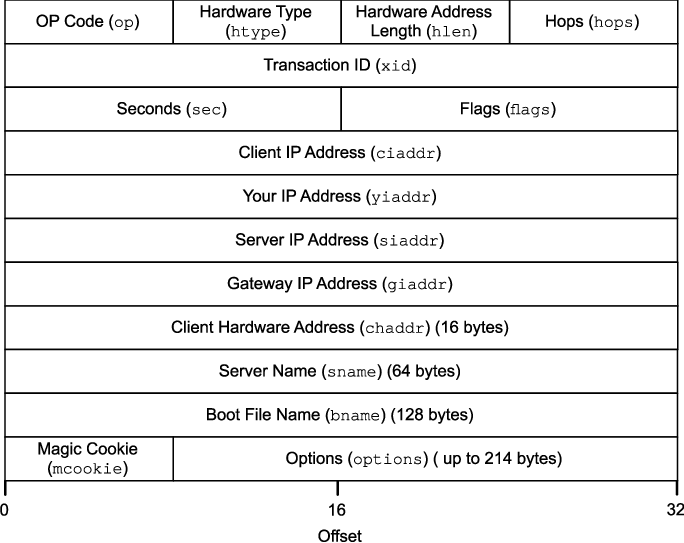
\includegraphics[scale=0.5]{Packet-format-for-DHCP.png}
		\\DHCP packet format\\
	\end{center}
	
	\subsubsection{Processing source IP}
	In order to get current utilization of an IP prefix, it has to be splitted in two parts: \emph{CIDR} and its IP part itself. 
	\emph{CIDR} is being used to calculate the maximum amount of hosts that this IP prefix can hold.
	The next step is to understand wheather source IP belong to the prefix or not. To find this out using source IP the network IP is being received.
	If this network ip is the same as the IP part of prefix, IP belongs to the prefix.

	\section{Implementation}
	This application was fully implemented in language C.
	\subsection{Receiving DHCP packets}
	In order to receive DHCP packets and their data, header \verb|<pcap.h>| is used. Implementation of obtaining packets slightly differs depending on method with which DHCP packets are being provided.
	\subsubsection{Receiving from an network interface}
	To successfully receive data from an interface, firstly, pcap handler needs to be opened on that network interface with \verb|pcap_open_live()|.
	Then application will continuously catch dhcp packets using function \verb|pcap_loop()| and pass them further, this process will be interrupted with \emph{CTRL + C} combination or if utilization of a prefix will reach 100\%.
	\subsubsection{Receiving from pcap file}
	Same as working with interface, to obtain data from a file, it is being opened using function \verb|pcap_open_offline()|.
	After that data will be processed until file ends or program will be interrupted.
	\subsection{Processing packet data}
	To extract source IP from the packet and to process it further, is used \verb|struct in_addr|, from the header \verb|<arpa/inet.h>|, and its functions.
	With help of several functions from \verb|<string.h>| IP prefix is being splitted into two parts and then using bitwise operations is being checked if IP coresponds to a prefix.\cite{string}
	\subsection{Output}
	Every time new packet was processed, updated information is printed to the output. If application runs on a specidied interface, it can be considered as a console application.
	In that case output is executed using header \verb|<ncurses.h>|, information about IP prefixes will be printed out as soon as first packet will be received\cite{ncurses}. 
	If data is being read from pcap file, the output will be done after all data from the file was processed.
	If utilization of a prefix exceeds 50\%, information about this is printed to the log using \verb|<syslog.h>|.\cite{Syslog}

	\section{Instructions for use}
	After unzipping tar archive with the project, compile code with command \verb|make|. Executable file dhcp-stats will be created.
	It can be runned using the following command:
	\begin{center}
		\verb|./dhcp-stats [-r <filename>] [-i <interface-name>] <ip-prefix> [ <ip-prefix> [ ... ] ]|
	\end{center}
	\begin{itemize}
		\item \textbf{[-r <filename>]}: path to a pcap file.
		\item \textbf{[-i <interface-name>]}: network interface.
		\item \textbf{<ip-prefix> [ <ip-prefix> [ ... ] ]}: list of IP prefixes separated by a space. 
	\end{itemize}
	Interface or pcap file must be provided for the program to work but not both simultaneously. At least one IP prefix has to be given also.

	\newpage
	\addcontentsline{toc}{section}{\refname}
	\bibliographystyle{plain}
	\bibliography{bibliography}
\end{document}
